\chapter{Root Finding}\label{ch:root-finding}
 
\normalsize

Finding roots of a function is a ubiquitous mathematical procedure in physics. For example, an equilibrium position of a particle in a potential field is determined as the place where the net force is zero, i.e., $U'(x)=0$. In many cases, the equation is transcendental and no analytical solution is available. Even when analytical solutions are known, numerical evaluation of them may suffer from the round-off error.  In this chapter,  we discuss how to find a root of a given equation $f(x)$ within acceptable error $\epsilon$ (tolerance). There are various methods depending on available information. If the derivative of the function is known, some methods definitely utilize it. Other methods do not require the derivative and use other information.  We need to choose a good algorithm for a given situation.

\noindent
\section{Quadratic, Cubic, and Quartic Polynomials}

The roots of quadratic, cubic and quartic polynomials can be expressed in analytic expressions and we just evaluate them numerically. However, in some extreme cases, numerical errors become too large and a special care must be taken.

\noindent
\subsection{Quadratic Polynomials}

The roots of quadratic equation:
\begin{equation}
a x^2 + b x + c = 0, \qquad a \neq 0
\end{equation}
are well known as
\begin{equation}\label{eq:roots_quadratic}
x_{1,2} = \frac{-b \mp \sqrt{b^2 - 4 a c}}{2 a}
\end{equation}
However, when $ac \ll b^2$, one of the solution suffers from the bit-off error as discussed in Chapter \ref{ch:numbers}.  Instead, the use of the following formula is recommended:
\begin{subequations}\label{ex:roots_quadratic}
\begin{equation}\label{eq:roots_quadratic+}
x_1 = \frac{-b - \sign(b)\sqrt{b^2 - 4 a c}}{2a}
\end{equation}
\begin{equation}\label{eq:roots_quadratic-}
x_2 = \frac{2c}{-b-\sign(b)\sqrt{b^2 - 4 a c}} = \frac{c}{a x_1}
\end{equation}
\end{subequations}
where the signum function $\sign(x)$ is defined by
					\[
					\sign(x) = \begin{cases} +1 & x>0 \\ -1 & x<0 \end{cases}
					\]
As demonstrated in Example \ref{ex:roots_quadratic}, these expressions do not suffer from the round-off error.

\begin{example}[Root of quadratic polynomials]\label{ex:roots_quadratic}

\begin{figure}
\centering
\includegraphics[width=3.3in]{04.root-finding/quadratic_root.pdf}
\caption{A root of the quadratic equation $\epsilon x^2+x+1/4=0$ is evaluated with two different methods with $\epsilon<1$. The left hand side of Eq. (\ref{eq:quad_trick2}) is initially approaching to the correct limit as $\epsilon$ decreases.  However, it goes erroneous below $\epsilon=10^{-5}$.  On the other hand, the right hand side steadily converges to the right answer.}
\label{fig:quadratic_root}
\end{figure}

\medskip
\noindent

In Eq. (\ref{eq:roots_quadratic+}), we used the equality.
\begin{equation}\label{eq:quad_trick2}
\frac{-b + \sqrt{b^2 - 4 a c}}{2a} = \frac{-2c}{b+\sqrt{b^2 - 4 a c}}
\end{equation}
When $|ac| \ll b^2$, the left hand side becomes numerically inaccurate.  On the other hand, the right hand side has no such problem.
We want to know how bad the left hand side is.  
Evaluate the both sides of the equality for $\epsilon x^2 + x + \displaystyle\frac{1}{4} = 0$ where $\epsilon = 0.1, 0.01, \cdots$. Reduce the value of $\epsilon$ until it hits the machine epsilon. Note that the exact answer for $\epsilon=0$ is $x=-\displaystyle\frac{1}{4}$.  Which side of Eq. (\ref{eq:quad_trick2}) approaches to the correct limit?  Program \ref{prog:quad_trick} evaluate the both sides of Eq. (\ref{eq:quad_trick2}). The results are plotted in Fig. \ref{fig:quadratic_root}.  The left hand side of Eq. (\ref{eq:quad_trick2}) is initially approaching to the correct limit as $\epsilon$ decreases.  However, it goes erroneous below $\epsilon=10^{-5}$.  On the other hand, the right hand side 
steadily converges to the correct answer.   (This example is a solution to Problem \ref{ch:numbers}.1.)
\end{example}

\noindent
\subsection{Cubic Polynomials}\label{sec:roots_cubic}

The roots of cubic polynomial
\begin{equation}\label{eq:cubic}
a x^3 + b x^2 + c x + d = 0, \quad a \ne 0
\end{equation}
can be obtain analytically. There  are various mathematical descriptions of the solutions but most of them are not convenient for numerical calculations. The following procedure is simple and does not use complex numbers.\cite{cubic_roots} Without losing generality, we can assume $a=1$. [The roots do not change if Eq (\ref{eq:cubic}) is divided by $a$.]

First, we evaluate the following quantities: 
\begin{equation}
F  = \frac{3 c - b^2}{3}, \quad
G  = \frac{2 b^3 - 9 b c + 27 d}{27}, \quad
H  = \frac{G^2}{4} + \frac{F^3}{27}
\end{equation}
where $H$ is a discriminant for Eq. (\ref{eq:cubic}).
If $H<0$, then there are three real roots:
\begin{equation}
x_1 = P + 2 J M, \qquad
x_2 = P - J (M+N), \qquad
x_3 = P - J (M-N)
\end{equation}
where 
\begin{align}
I &= \sqrt{\frac{G^2}{4} - H}, & J &= \sqrt[3]{I}, &K &= \arccos(-G/2I) \nonumber\\
M &= \cos(K/3), & N &= \sqrt{3} \sin(K/3), & P &= -\frac{b}{3} \, .
\end{align}
If $H=0$, the above solutions are still valid but two of solutions are degenerate.
If $H>0$, then there is one real root and two others are complex:
\begin{equation}
x_1 = S+U-\frac{b}{3}, \quad x_{2,3} = -\frac{S+U}{2} - \frac{b}{3} \pm i \frac{(S-U)\sqrt{3}}{2}
\end{equation}
where
\begin{equation}
S = \sqrt[3]{\sqrt{H}-\frac{G}{2}}, \quad U =  -\sqrt[3]{\sqrt{H}+\frac{G}{2}}
\end{equation}

In some cases, we don't get a good result due to the round-off error.  Use an iterative method explained in Section \ref{sec:iterative-root-finding} to see if the round-off error is small enough. Since the numerical results obtained by the present method is already close to the exact one, the iterative method should converge quickly (a few iterations are enough for most cases).


\nopagebreak[4]
\begin{example}[Cubic Polynomials]\label{ex:roots_cubic}

\nopagebreak[4]
\noindent
Let's try to find all roots of $x^3 -9 x^2 + 23 x + 15=0$ using the formula given above.  It can be factorized to $(x-1)(x-3)(x-5)=0$ and thus the exact solution is $x=$ 1, 3, and 5. Program \ref{prog:roots_cubic} finds them correctly.

\begin{mybox}
\small
\begin{verbatim}
Answer = 1.00000,  3.00000,  5.00000
\end{verbatim}
\normalsize
\end{mybox}
\end{example}

\subsection{Quartic Polynomials}

The roots of quartic polynomial
\begin{equation}
a x^4 + b x^3 + c x^2 + d x + e = 0
\end{equation}
can be also solved analytically.  Assuming $a=1$ as before, we evaluate the following quantities:
\begin{equation}
F  =- \frac{3 b^2}{8}  + c , \quad
G  = \frac{b^3}{8} - \frac{b c}{2} + d, \quad
H  = - \frac{b^4}{256} + \frac{b^2 c}{16} - \frac{b d}{4} + e
\end{equation}
If $G=0$, then the four roots are
\begin{equation}
x_{1,2,3,4} = -\frac{b}{4} \pm \sqrt{\frac{-F \pm \sqrt{F^2-4H}}{2}}
\label{eq:quartic_roots1}
\end{equation}
If $G \neq 0$, then
\begin{subequations}
\begin{equation}
x_{1,2} = -\frac{b}{4} + \frac{W \pm \sqrt{-\left (3F + 2Y + \frac{2G}{W}\right )}}{2}
\end{equation}
\begin{equation}
x_{3,4} = -\frac{b}{4} - \frac{W \pm \sqrt{-\left (3F + 2Y - \frac{2G}{W}\right )}}{2}
\end{equation}
\label{eq:quartic_roots2}
\end{subequations}
where
\begin{equation}
Y = \begin{cases}
-\displaystyle\frac{5F}{6} + U - \frac{P}{3U} & \text{if } U \ne 0 \\
\\
-\displaystyle\frac{5F}{6} - \sqrt[3]{Q} & \text{if } U=0
\end{cases}, \qquad  W = \sqrt{H+2Y} 
\end{equation}
\begin{equation}
P = -\frac{F^2}{12}-H, \qquad Q = -\frac{F^3}{108} + \frac{F H}{3} - \frac{G^2}{8}, \qquad  U = \sqrt[3]{- \frac{Q}{2}\pm \sqrt{\frac{Q^2}{4}+\frac{P^3}{27}}}
\end{equation}

Similar to quadratic and cubic equations, sever round-off error can happen, for example, when $H \ll F$ in Eq (\ref{eq:quartic_roots1}). Use an iterative method to improve the results.

\section{Iterative Methods}\label{sec:iterative-root-finding}

In this section, we solve $f(x)=0$ for $x$ where $f(x)$ is a continuous function.  There may be multiple solutions.  Any root finding method needs a rough idea of the location of root you are looking for.  The first step is to \emph{bracket} the target root $x^*$ between $x_\textsc{l}$ and $x_\textsc{u}$ such that $x_\textsc{l} < x^* < x_\textsc{u}$.  It is important that there is only one root between $x_\textsc{l}$ and $x_\textsc{u}$.  It turns out that this is not an easy task for computer. Searching is something difficult even for computers to accomplish. On the other hand, human eyes can find the bracket easily if you are able to plot the function.  Computers do not have an eye to view the whole curve.  Therefore, the best practice is to plot the function and bracket the target root by visual inspection.  However, in some cases it is desirable to have a robust numerical method to find the bracket. For example,  when root finding is required many times during long computer simulation, you can't stop the simulation to visually inspect the bracket.   There are simple algorithms of finding the bracket\cite{numerical_recipes} but unfortunately no method guarantees the outcome.   In this chapter, we assume that the bracket is done by direct visual inspection.

Any iterative method needs a criteria to stop the iteration. Ultimately, we stop it when the error is smaller than the tolerance.  However, in practice we never know the exact error.  If we knew it, we have the exact root! Therefore, we must carefully choose an ending criteria.

\subsection{Bisection method}

\begin{figure}
\begin{minipage}{0.47\linewidth}
\centerline{\includegraphics[width=2.5in]{04.root-finding/bisection.pdf}}
\caption{Bisection method. Starting with initial bracket $(x_0, x_1)$, the bracket is at each iteration halved to $(x_2,x_1)$, $(x_2,x_3)$, $(x_2, x_4)$, $(x_5, x_4)$, $\cdots$.}\label{fig:bisection}
\end{minipage}
\hfill
\begin{minipage}{0.47\linewidth}
\centerline{\includegraphics[width=2.5in]{04.root-finding/newton-raphson.pdf}}
\caption{Newton-Raphson method. Starting with initial guess $x_0$, the line tangent to the curve at the current point $x_n$ is used to find a new imroved root $x_{n+1}$.  If the initial guess $x_0$ is close enough to the true root, this procedure rapidly converges to it.}\label{fig:newton-raphson}
\end{minipage}
\end{figure}

Suppose we evaluate the function at two different points $x_\textsc{l}$ and $x_\textsc{u}$.  If $f(x_\textsc{l}) f(x_\textsc{u}) < 0$, then we are sure that there is at least one root between the two points.  This is a sufficient condition but not a necessary condition.  When there is no root between the bracket, $f(x_\textsc{l}) f(x_\textsc{u}) >0$.  However, when there are even number of roots in the bracket, the same inequality is valid.  In the following we assume that a good bracket is found by visual inspection or other means so that there is only one root within the bracket. 

Consider a mid point $x_\textsc{m}$ between  $x_\textsc{l}$ and $x_\textsc{u}$.  If $f(x_\textsc{l}) f(x_\textsc{m}) < 0$, the root must be between $x_\textsc{l}$ and $x_\textsc{m}$.  Now we have a new bracket $x_\textsc{l}$ and $x_\textsc{m}$.  Otherwise, the root must be between $x_\textsc{m}$ and $x_\textsc{u}$, which is the new bracket.  Repeating this procedure, the root is isolated in a small region. The error must be smaller than $x_\textsc{u}-x_\textsc{l}$ and thus the iteration is terminated when $x_\textsc{u}-x_\textsc{l} < \text{tolerence}$. This is the method of bisection.  Figure \ref{fig:bisection} demonstrate how the bisection method works. 
The procedure of this iterative method is  as follows.

\bigskip
\begin{center}
	\begin{myalgobox}
		\Algorithm{Bisection method}\label{argo:bisection}
		
				\begin{minipage}{5.5in}
					\begin{enumerate}
\item Get a initial bracket $x_\textsc{l}$ and $x_\textsc{u}$ and a tolerance $\epsilon$.
\item Make it sure that $f(x_\textsc{l}) f(x_\textsc{u}) <0$.  Otherwise, stop and check the initial bracket.
\item Evaluate the function at the mid point $x_\textsc{m} = \frac{1}{2}(x_\textsc{l}+x_\textsc{u})$.
\item If $x_\textsc{u} - x_\textsc{l}< \epsilon$, $x_\textsc{m}$ is the root and stop here.  Otherwise continue.
\item If $f(x_\textsc{l}) f(x_\textsc{m}) < 0$, then the root is between $x_\textsc{l}$ and $x_\textsc{m}$.  Let $x_\textsc{u}=x_\textsc{m}$ and go to step 3.  Otherwise continue.
\item The root must be between $x_\textsc{m}$ and $x_\textsc{u}$.  Let $x_\textsc{l}=x_\textsc{m}$ and go to Step 3.
                    \end{enumerate}
                \end{minipage}
\end{myalgobox}
    \end{center}

This method  is generally robust and steadily approaches to the root. However, it is not a smart one and iterates many times before reaching the root.  
This method fails when the root is located at the edge of support since the root cannot be bracketed. For example, the bisection method is not able to solve $\sqrt{x-a}=0$ simply because the function cannot be evaluated for $x<a$. It turns out that not only the bisection method but many other methods also fail for this function.

\bigskip
\begin{example}[Bisection Method]\label{ex:bisection}
Find a root of $x^3 -9 x^2 + 23 x + 15=0$ between $x_1=1.5$ and $x_2=4$. 
Program \ref{prog:bisection} implement the above Bisection algorithm.  With tolerance $10^{-6}$, the bisection method converges to a root after 20 iterations. The root agrees with the exact answer. (See Example \ref{ex:roots_cubic}.)
\begin{mybox}
\small
\begin{verbatim}
Answer = 3.00000  (iteration= 20)
\end{verbatim}
\normalsize
\end{mybox}
\end{example}

\noindent
	\exercise
	Find two other roots.
	
	\bigskip\noindent
	\exercise
	Find all roots using $x_\textsc{U}-x_\textsc{L}$ as the measure of error.
	
\noindent
\subsection{Newton-Raphson method}

If the derivative of the function is known, there are faster methods utilizing it.  Newton-Raphson method is one of those. Starting with an initial guess $x_0$, we approximate the function using Taylor expansion
\begin{equation}
f(x) = f(x_0) + f'(x_0) (x-x_0) + \frac{1}{2} f''(x_0) (x-x_0)^2 + \cdots 
\end{equation}
If $x_0$ is close to the root, we can ignore the higher order terms.  Keeping only the first order term, the original equation $f(x)=0$ is replaced by
\begin{equation}
f(x_0) + f'(x_0) (x-x_0) = 0
\end{equation}
and the root of this approximted equation is 
\begin{equation}
x_1 = x_0 - \frac{f(x_0)}{f'(x_0)}
\end{equation}
which should be closer to the root than $x_0$.  Repeating this procedure, we have a recursive equation
\begin{equation}
x_{n+1} = x_n - \frac{f(x_n)}{f'(x_n)}
\label{eq:newton_raphson}
\end{equation}
We stop the iteration when $|x_{n+1}-x_n| < \epsilon \text{ (tolerance)}$.  Is this a reasonable criteria?  Using Taylor expansion around $x_n$,
\begin{equation}
f(x^*) = f(x_n) + (x^*-x_n) f'(x_n)
\end{equation}
where $x^*$ is the exact root.   By definition, $f(x^*)=0$.  Then, the error is given by $|x^*-x_n| =  \left | \displaystyle\frac{f(x_n)}{f'(x_n)} \right | = |x_{n+1}-x_n|$.  As long as $x_n$ is close to $x^*$, the criteria measures the error correctly.

Note that this method does not require initial bracketing.  However, 
this method works great only if the initial point is sufficiently close to the root. Otherwise it is not guaranteed to converge to the target root.  It might reach another root which you are not looking for. 
In order to avoid this failure, find a reasonably accurate root using the bisection method and switch to the Newton-Raphson method for the further improvement.  While the bisection method is relatively robust many iterations are needed.  On the other hand, the Newton-Raphson method converges faster.  Therefore, such a hybrid method make a sense. 

\bigskip
\begin{myalgobox}
		\Algorithm{Newton-Raphson method}\label{argo:newton-raphson}
				
				\begin{minipage}{5.5in}
					\begin{enumerate}
						\item Set a tolerance $\epsilon$.
						\item Choose an initial guess $x_{0}$ and let $n=0$.
						\item Estimate a new candidate by $x_{n+1} = x_n - \displaystyle\frac{f(x_n)}{f'(x)}$.
						\item If $|x_{n+1}-x_n| < \epsilon$, then $x_{n+1}$ is the root.  Stop the iteration.
						\item If not, increment $n$ and go to step 3.
					\end{enumerate}
				\end{minipage}
\end{myalgobox}

\noindent
\exercise
The solution to $\sqrt{x-a} = 0$ is $x=a$.  Can we find it by the Newton-Raphson method?  Starting with $x_0 > a$, try to find $x_1$ and $x_2$. Verify that $x_2$ does not exist.



\subsection{Secant method}

The Newton-Raphson method requires the analytic expression of the first order derivative, which limits the range of applications. However, the same idea can be used without the analytic expression.  If we replace the analytic derivative with the numerical derivative, the Newton-Raphson procedure still works.  Using the backward finite difference method [Eq. \eqref{eq:diff_bwd}], the recursive equation (\ref{eq:newton_raphson}) becomes
\begin{equation}
x_{n+1} = x_n - \frac{x_{n}-x_{n-1}}{f(x_n)-f(x_{n-1})} f(x_n)
\end{equation}
This method is commonly known as the secant method. Use the bisection method before starting the secant method to ensure the convergence.

One problem is that this method needs two points to start the iteration. However, this is not a big issue since we can pick any point close to the initial guess. If the root is already bracketed between $a$ and $b$, use $x_1 = x_0 + \Delta$ with $\Delta \ll b-a$. If the secant method is preceded by the bisection method, use the final bracket from the bisection calculation.  Then, $\Delta = (b-a)/10$ is good enough.

\bigskip
\begin{myalgobox}
		\Algorithm{Secant method}\label{argo:secant}

				\begin{minipage}{5.5in}
					\begin{enumerate}
						\item Find bracket $a$ and $b$. Set a tolerance $\epsilon$. 
						\item Choose two initial points
						$x_0$ and $x_1 = x_0 + \displaystyle\frac{b-a}{10}$ and let $n=1$
						\item Estimate a new candidate by $x_{n+1} = x_n - \displaystyle\frac{x_n-x_{n-1}}{f(x_n)-f(x_{n-1})} f(x_n)$.
						\item If $|x_{n+1}-x_n| < \epsilon$, then $x_{n+1}$ is the root.  Stop the iteration.
						\item If not, increment $n$ and go to step 3.
					\end{enumerate}
				\end{minipage}
\end{myalgobox}

\begin{figure}
\centerline{\includegraphics[width=3in]{04.root-finding/cos3x_sinx.pdf}}
\caption{The function used in Example \ref{ex:cos3x_sinx}.  The smallest positive root is bracketed between 0.2 and 0.8 (between the dashed lines) by visual inspection.}
\label{fig:cos3x_sinx}
\end{figure}

\vspace{18px}
\begin{example}[Multiple roots]\label{ex:cos3x_sinx}

\medskip
Find the smallest positive root of $f(x)=\cos 3x \sin x$.  Since 
this function has infinitely many roots, we have to be careful about choosing an initial guess.
Figure \ref{fig:cos3x_sinx} plots the function.  By visual inspection, it is safe to say that the smallest positive root is between 0.2 and 0.8. We seek the solution with tolerance $\epsilon = 10^{-8}$.  If only the bisection method were used, it takes 24 iterations and the answer is 0.52359877.  

Program \ref{prog:newton-secant} runs 10 iterations of the bisection method
and the Newton-Raphson and Secant methods follow.  The output is shown below. The bisection method gets 0.52373047 which is close but not sufficient.  Subsequent Newton-Raphson method iterates only two times and obtained 0.52359878.  Similarly, the secant method also iterates twice and reaches the same answer as the Newton-Raphson.  
The exact answer is $\frac{\pi}{6} \approx 0.52359878$.  All methods arrive the correct answer. However,  the total number of iterations is 12 if the combination of the bisection and Newton-Raphson/secant methods is used, which is a half of the steps needed by the bisection method only.  For complicated equations, the time saving can be significant.
\begin{mybox}
\small
\begin{verbatim}
Bisection      = 0.52373047  (iteration= 10)
Newton-Raphson = 0.52359878  (iteration= 2)
Secant         = 0.52359878  (iteration= 2)
\end{verbatim}
\normalsize
\end{mybox}
\end{example}

\vspace{18px}
\noindent
\exercise
Find the second smallest positive root.

\newpage
\noindent
\section{Applications in Physics Problems}


\noindent
\subsection{Magnetic Phase Transition}

The Ising model explains the ferromagnetic phase transition.\cite{Ising}  Using the mean field approximation, the magnetization  per atom satisfies the following transcendental equation
\begin{equation}\label{eq:ising}
m = \mu \tanh \left ( \frac{C m}{\kB T} \right ) 
\end{equation}
where $C$ is a positive constant determined by the spin interaction between atoms, $T$ is temperature, and $\mu$ is the magnetic moment each spin carries.  We want to know the magnetization as a function of temperature by solving Eq. \eqref{eq:ising}.
By direct inspection $m=0$ is always a solution.  However, depending on temperature, there are more solutions. We want to plot all roots as functions of temperature.  First, we simplify the expression by introducing normalized magnetization $\tilde{m}=m/\mu$ and normalized temperature $\tilde{T}=\frac{\kB T}{\mu C}$. The normalized quantities are dimensionless and various constants disappear.  We omit tilde in the normalized quantities to avoid cluttering. Then, we solve
\begin{equation}
f(m) \equiv m - \tanh(m/T) = 0
\label{eq:ising2}
\end{equation}
utilizing its derivative
\begin{equation}
f'(m) = 1 - \frac{\sech^2 (m/T)}{T}
\end{equation}

To use the Newton-Raphson method, we need to start with a good initial guess.  As Fig \ref{fig:ising} shows, $\tanh(m) \rightarrow 1$ for $m \gg 1$.  Therefore, the root must be below $m=1$.  As $T$ approaches zero, the root approaches one.  Therefore, $m=1$ is a good starting point for low temperature case.  As temperature increases, the root gradually decreases toward zero.  Therefore, when temperature is lowered a little bit, the previous root can be a very good starting point of the next root finding process. We don't have to bracket the root in this case. 
The results are shown in Fig. \ref{fig:ising-bifurcation}.

\begin{figure}
\centering
	\begin{subfigure}{0.45\textwidth}
		\centering
		\includegraphics[width=2.5in]{04.root-finding/ising.pdf}
\caption{The magnetization is determiend by the crossing of $y=x$ and $y=\tanh(a x)$ where $a=1/T$. When $a<1$ $x=0$ is only the solution. For $a>1$, two more solutions appear.  $a=1$ corresponds to the critical point of the ferromagnetic transition.}\label{fig:ising-roots}
	\end{subfigure}
	\begin{subfigure}{0.45\textwidth}
		\centering
		\includegraphics[width=2.5in]{04.root-finding/ising-bifurcation.pdf}
\caption{Bifurcation of magnetization. For $T>1$ there is only one magnetic state $m=0$.  When temperature is lowered below a critical temperature $T_\textsc{C}=1$, two stable states, one with positive $m$ and the other with negative $m$.  $m=0$ is still a solution but unstable one. At $T=0$, the magnetization reaches the maximum possible value $m=\pm 1$ where all electrons have the same spin state.}{\label{fig:ising-bifurcation}}
	\end{subfigure}
\caption{Ferromagnetic Phase Transition}\label{fig:ising}
\end{figure}

\begin{example}[Bifurcation of magnetization]
Program \ref{prog:ising} finds the roots of Eq. (\ref{eq:ising}) by Newton-Raphson method and plots them. The result is shown in Fig. \ref{fig:ising-bifurcation}.  Above the critical temperature $S_\textsc{C}=1$, there is only one root and the magnetization vanishes.
Below $S_\textsc{C}$, positive and negative magnetization spontaneously appear.  The root at $m=0$ still exists but it is no thermodynamically not stable. 
\end{example}

\vspace{18px}
\noindent
\exercise[Spontaneous vs induced magnetization]

When external magnetic field  $H$ is applied, the mean-field equation becomes
\begin{equation}
m = \mu \tanh \left (\frac{\mu H + C m}{\kb T} \right )\, .
\end{equation}
Modify Program \ref{prog:ising} and plot the magnetization as a function of temperature with a fixed value of $H \ne 0$.  Try various different values of $H$.  How is the spontaneous magnetization shown in Fig. \ref{fig:ising-bifurcation} modified by the magnetic field?
[Use the normalized magnetic field $\tilde{H} = H/C$.]


\noindent
\subsection{Energy of a Quantum Particle in a Square Potential}\label{sec:quantum-well}


A particle of mass $m$ is trapped in a square well potential of depth $V_0$ and width $2a$.  Energy eigenvalue $E$ is determined by Sch\"{o}dinger equation
\begin{equation}
\left [ -\frac{\hbar^2}{2m} \frac{\md^2}{\md x^2} + V(x) \right ] \psi(x) = E \psi(x)
\end{equation}
Analytical calculation ends up with the following transcendental equations\cite{square_well}
\begin{subequations}\label{eq:square_well}
\begin{eqnarray}
z \tan(z) - \sqrt{z_0^2 - z^2} &=& 0 \qquad \text{for symmetric states} \label{eq:square_well_symmetric} \\
z \cot(z) + \sqrt{z_0^2 - z^2} &=& 0 \qquad \text{for anti-symmetric states}\label{eq:square_well_antisymmetric}
\end{eqnarray}
\end{subequations}
where
\begin{subequations}
\begin{eqnarray}
z &=& \sqrt{\frac{2 m a^2 E}{\hbar^2}} \\
z_0 &=& \sqrt{\frac{2 m a^2 V_0}{\hbar^2}}
\end{eqnarray}
\end{subequations}
The roots of Eqs (\ref{eq:square_well}) determines the energy eigenvalues. WE want to know all eigenvalues. However, the number of roots depends on the system parameters, which makes it difficult to bracket a root.  We need to inspect the location of the roots. In Fig. the left hand side of Eq (\ref{eq:square_well_symmetric}) is plotted. First of all, we note that the function is defined for $z \in (0, z_0)$ and thus all roots must be between $0$ and $z_0$.  Considering $\tan x$ diverges at $2\pi (n \pm 1/4)$, each root must be between the diverging points.
Hence, we bracket the roots in $(0,\frac{\pi}{2}-\delta)$, $(\frac{\pi}{2}+\delta, \frac{3\pi}{2}-\delta)$, $\cdots$, $2\pi(n+\frac{1}{4})+\delta, z_0)$.  Here $\delta$ is a small positive quantity to avoid the singularities. Program \ref{prog:square_well}  finds all roots for given $z_0$. Ten iterations of the bisection methods followed by the secant method find two roots.

\begin{center}
\begin{minipage}{0.5\textwidth}
\small
\begin{Verbatim}[frame=single]
root=1.34475105
root=3.98582621
\end{Verbatim}
\normalsize
\end{minipage}
\end{center}

\begin{figure}
\centering
	\begin{subfigure}{0.45\textwidth}
		\centering
		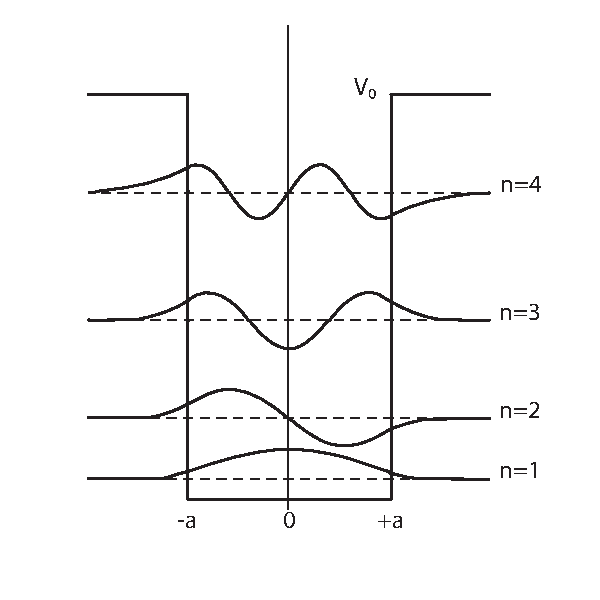
\includegraphics[width=2.2in]{04.root-finding/square_well_energy.pdf}
\caption{A square well potential with depth $V_0$ and width $2a$.  Two symmetric and two anti-symmetric energy eigenstates are plotted.}\label{fig:square_well_energy}
	\end{subfigure}
	\begin{subfigure}{0.45\textwidth}
		\centering
		\includegraphics[width=2.5in]{04.root-finding/square_well_root.pdf}
\caption{The left hand side of Eq (\ref{eq:square_well_symmetric}) is plotted for $z_0=6$. There are two roots. Clearly the root is bracketed by the dashed lines at $x=\frac{\pi}{2}$ and $\frac{3\pi}{2}$.}\label{fig:square_well_root}
	\end{subfigure}
\caption{Quantum particle in a finite suare well}\label{fig:square_well}
\end{figure}

\noindent
\subsection{Classical Turning Points}

In Section  \ref{sec:oscillation1}, we tried to calculate the period of oscillation but we were not quite ready at that time because we did not know how to find the turning points.  Now we can find them using a numerical root finding method. 
Suppose that a particle is bound in a potential
\begin{equation}
U(x) = U_0 \left [ \sin \left ( \frac{2\pi x}{L} \right )- \frac{1}{4} \sin \left ( \frac{4\pi x}{L}\,. \right ) \right ]
\label{eq:ratchet_potential}
\end{equation}
We want to find the period of the bound motion using the formula 
\eqref{eq:oscillation-period}.
The turning points are the roots of $U(x)=E$. The potential is simple and we can find the analytic expression of its derivative.  Hence, the Newton-Raphson method can be used to find the roots.

\vspace{18px}
\noindent
\exercise
Modify Program \ref{prog:newton-secant} and find a pair of the classical turning points of the potential (\ref{eq:ratchet_potential}).
Using the results, find the period of oscillation.

\noindent
\subsection{Closest Approach in Scattering}

In Section \ref{sec:scattering1},
we discussed how to evaluate the scattering angle \eqref{eq:phi_r}.  In order to carry out the integral, we still have to find the closest approach $r_0$ determined by 
Eq. \eqref{eq:root_r}.
For the screened Coulomb potential, we are able to calculate the first order derivative of the equation.  The Newton-Raphson method seems a good choice.

\vspace{18px}
\noindent
\exercise
Solve Eq.  \eqref{eq:root_r} for the Yukawa potential.  Then, calculate the scattering angle, Eq. \eqref{eq:phi_r}, using the method discussed in Section \ref{sec:scattering1}.

\vfill
\noindent
\section{Problems}

\begin{enumerate}[labelwidth=0.5cm,labelindent=0cm,leftmargin=*,label=\bfseries \thechapter.\arabic*,align=left]
\item
The interaction energy between two atoms is often described by the Morse potential\cite{morse_potential}
\begin{equation}
U(r) = D_e \left [\me^{-2 (r-r_0)/a} - 2 \me^{-\alpha (r-r_0)/a} \right ]
\end{equation}
where $r$ is the distance between the atoms.  The parameters, $D_e$. $r_0$, and $a$ are, dissociation energy, equilibrium distance, and the range of interaction, respectively. To simplify numerical calculation, we normalize energy and distance by $D_e$ and $a$. In addition, we use the displacement from the equilibrium position as the coordinate.  Then, the potential is simply
\begin{equation}
U(x) = \me^{-2x}-2 \me^{-x}\,.
\end{equation}
were $x=(r-r_0)/a$.
Find the classical turning points for $E=-0.5$ (This means the actual energy is $E=-D_e/2$ since we use $D_e$ as the unit of energy.)
Do not forget to plot the potential and visually inspect the turning point before using numerical root finding methods.
\item
Find the eigenvalue of all asymmetric state by solving Eq. (\ref{eq:square_well_antisymmetric}) for $z_0=6$.

\item
A quantum ball of mass $m$ is bouncing on a hard floor under a uniform gravity $g$.\cite{qm_bounce}  Schr\"{o}dinger equation for the particle is
\begin{equation}
-\frac{\hbar^2}{2m} \frac{\md^2 \psi(y)}{\md y^2} + m g y\, \psi(y) = E \psi(y).
\label{eq:bouncing_ball}
\end{equation}
The wavefunction $\psi$ must vanish at the floor (boundary condition).  To find the energy eigenvalue, we first simplify the Schr\"{o}dinger equation. Introducing a new variable $z= \alpha (y-E/mg)$ where
\begin{equation}
\alpha = \left ( \frac{2 m^2 g}{\hbar^2} \right )^{1/3}
\end{equation}
Eq. (\ref{eq:bouncing_ball}) is rewritten as
\begin{equation}
\frac{\md^2 \psi(z)}{\md z^2} = z \psi(z)\,
\end{equation}
This equation is known as Airy equation and its solution is Airy function $\text{Ai}(z)$.  Hence, the energy eigenfunction is
$\psi(z) = N\, \text{Ai}(z)$ where $N$ is a normalization constant.  Now, we apply the boundary condition.   At $y=0$. $z=-\alpha E/mg$ and thus $\text{Ai}(-\alpha E/mg)=0$.  This boundary condition indicates that the energy $E$ is determined by the roots of the Airy function. 
Denoting the $n$-th root as $z_n$, the energy is $E_n=- m g z_n /\alpha$.  The bouncing quantum ball has discrete energy!
Find the smallest root of the Airy function and corresponding energy $E_1$.
Use the built-in Airy function $\texttt{airy()}$ in MATLAB.  For C or Fortran, GNU Scientific Library (GSL)\footnote{You can find GSL at 
\texttt{https://www.gnu.org/software/gsl/}.} provides Airy function.
\end{enumerate}

\newpage
\section*{MATLAB Source Codes}
\addcontentsline{toc}{section}{\protect\numberline{}MATLAB Source Codes}


\bigskip\noindent
\program
\label{prog:quad_trick}

\footnotesize
\begin{verbatim}
%**************************************************************************
%*     Example  4.1                                                       *
%*     filename: ch04pr01.m                                               *
%*     program listing number: 4.1                                        *
%*                                                                        *
%*     This program finds roots of a quadratic equation                   *
%*               a x^2 + x + 1/4 = 0                                      *
%*     for which the quadratic equation formula                           * 
%*            x = (-1 + sqrt(1 - a))/(2a)                                 *
%*     fails for small value of a.                                        *
%*                                                                        *
%*     Programed by Ryoichi Kawai for Computational Physics Course.       *
%*     Last modification:  10/13/2013.                                    *
%**************************************************************************
clear all;

b=1;  % fixed parameters
c=0.25;

n=1;
a(1)=1;
while (a>eps())
  d = b^2-4*a(n)*c;
  x1(n) = (-b+sqrt(d))/(2*a(n));
  x2(n) = -2*c/(b+sqrt(d));
  fprintf('a= %22.16e, lhs=%22.16e, rhs=%22.16e \n',a(n),x1(n),x2(n));
  n=n+1;
  a(n)=a(n-1)/10;
end

% plot the results
p=loglog(a(1:n-1),abs(x2+0.25),'o',a(1:n-1),abs(x1+0.25),'s');
set(p(1),'Linewidth',2,'Color','red')
set(p(2),'Linewidth',2,'Color','blue')
xlabel('a','Fontsize',14)
ylabel(texlabel('|x - x_0|'),'Fontsize',14)  % x_0 = root at a=0
legend('lhs','rhs')
legend('Location','Southeast')
\end{verbatim}
\normalsize

\ruleend

\bigskip\noindent
\program
\label{prog:roots_cubic}
\footnotesize
\begin{verbatim}
%**************************************************************************
%*     Example  4.2                                                       *
%*     filename: ch04pr02.m                                               *
%*     program listing number: 4.2                                        *
%*                                                                        *
%*     This program finds roots of a cubic equation                       *
%*               a*x^3 + b*x^2 + c*x + d = 0                              *
%*                                                                        *
%*     Programed by Ryoichi Kawai for Computational Physics Course.       *
%*     Last modification:  10/13/2013.                                    *
%**************************************************************************
clear all;

% coefficients
b=-9; c=23; d=-15;

% formula for cubic polynomials
F=(3*c-b^2)/3;
G=(2*b^3 - 9*b*c + 27*d)/27;
H=G^2/4 + F^3/27;

yes = false;

if H>0
    S= (sqrt(H)-G/2)^(1./3.);
    U=-(sqrt(H)+G/2)^(1./3.);
    x = S+U-b/3;
    fprintf('Answer = %.5f\n',x);

else
    I=sqrt(G^2/4-H);
    J=I^(1./3.);
    K=acos(-G/(2*I));
    M=cos(K/3);
    N=sqrt(3)*sin(K/3);
    P=-b/3;    
    x(1) = P-J*(M+N);
    x(2) = P-J*(M-N);
    x(3) = P+2*J*M;
    fprintf('Answer = %.5f,  %.5f,  %.5f \n',x);
end
\end{verbatim}
\normalsize

\ruleend

\program
\bigskip\noindent
\label{prog:bisection}
\footnotesize
\begin{verbatim}
%**************************************************************************
%*     Example  4.3                                                       *
%*     filename: ch04pr03.m                                               *
%*     program listing number: 4.3                                        *
%*                                                                        *
%*     This program finds roots of a cubic equation                       *
%*               a*x^3 + b*x^2 + c*x + d = 0                              *
%*     using the bisection method.                                        *
%*                                                                        *
%*     Programed by Ryoichi Kawai for Computational Physics Course.       *
%*     Last modification:  01/24/2018.                                    *
%**************************************************************************
clear all;

% define a cubic equation
b = -9;
c = 23;
d =-15;

f = @(x) x^3+b*x^2+c*x+d;

% tolerance
epsilon=input('Enter tolerance =');

% initial bracket
x1=1.5;
x2=4;
f1 = f(x1);
f2 = f(x2);

% iteration counter
n=0;

% mid point
xm = (x1+x2)/2;
fm = f(xm);
while abs(fm) > epsilon
    if f1*fm < 0  % root in the lower half
        x2=xm;
        f2=fm;
    else          % root in the upper half
        x1=xm;
        f1=fm;
    end
    xm = (x1+x2)/2;  % new mid point
    fm = f(xm);
    n=n+1;
end

fprintf('Answer = %.5f  (iteration= %i)\n',xm,n);
\end{verbatim}

\normalsize


\ruleend

\bigskip\noindent
\program
\label{prog:newton-secant}
\footnotesize
\begin{verbatim}
%**************************************************************************
%*     Example 4.4                                                        *
%*     filename: ch04pr04.m                                               *
%*     program listing number: 4.4                                        *
%*                                                                        *
%*     This program seeks the root of                                     *
%*             cos(3*x)*sin(x)=0                                          *
%*     between x=0.2 and 0.8 using bisection, Newton-Raphson, and         *
%*     secant methods.                                                    *
%*                                                                        *
%*     Programed by Ryoichi Kawai for Computational Physics Course        *
%*     Revised on 01/07/2014.                                             *
%**************************************************************************
clear all;

% define function and its derivative
f=@(x) cos(3*x)*sin(x);
df=@(x) -3*sin(3*x)*sin(x) + cos(3*x)*cos(x);

% initial bracket
x1=0.2;
x2=0.8;
f1=f(x1);
f2=f(x2);
if f1*f2 > 0
   error('Bracket is incorrect');
end

% tolerance
epsilon=1e-8;

% bisection 10 iterations

% iteration counter
n=0;

% Bisection method (10 iterations)
xm = (x1+x2)/2;
fm = f(xm);
while n<10
    if f1*fm < 0  % root in the lower half
        x2=xm;
        f2=fm;
    else          % root in the upper half
        x1=xm;
        f1=fm;
    end
    xm = (x1+x2)/2;  % new mid point
    fm = f(xm);
    n=n+1;
end

fprintf('Bisection      = %.8f  (iteration= %i)\n',xm,n);

% Newton-Raphson method
x = xm;
fx = fm;
n = 0;
while abs(fx)> epsilon
    dfx = df(x);
    x = x - fx/dfx;
    fx = f(x);
    n = n+1;
end

fprintf('Newton-Raphson = %.8f  (iteration= %i)\n',x,n);

% Secant method
dx = (x2-x1)/10;
x1 = xm;
f1 = fm;
x2 = x1 + dx;
f2 = f(x2);
n = 0;
while abs(f2)> epsilon
    x = x2 - (x2-x1)/(f2-f1)*f2;
    x1 = x2;
    f1 = f2;
    x2 = x;
    f2 = f(x);
    n = n+1;
end

fprintf('Secant         = %.8f  (iteration= %i)\n',x,n);
\end{verbatim}
\normalsize

\ruleend

\bigskip\noindent
\program
\label{prog:ising}
\footnotesize
\begin{verbatim}
%**************************************************************************
%*     Example 4.5                                                        *
%*     filename: ch04pr05.m                                               *
%*     program listing number: 4.5                                        *
%*                                                                        *
%*     This program calculates magnetization as a function of             *
%*     temperature using the mean field Ising model:                      *
%*         x = x tan(x/S)                                                 *
%*     where the variables are normalized as                              *
%*         x = m/m_0 and S=k*T/(C*m_0) .                                  *
%*                                                                        *
%*     Programed by Ryoichi Kawai for Computational Physics Course        *
%*     Revised on 01/07/2014.                                             *
%**************************************************************************
clear all;
N=101; % number of data points
tol=10^(-6);  % tolerance

dS = 2/(N-1); % step size in temperature

for i=1:N
    S=(i-1)*dS;  % temperature
    a=1/S;
    f=@(x) x - tanh(a*x);  % function
    df=@(x) 1 - a*sech(a*x)^2;  % derivative
    % Newton-Raphson method
    x=2;  % initial guess
    fx=f(x);
    while fx>tol
      x=x-fx/df(x);
      fx=f(x);
    end
    % store the magnetization and temperature  
    m(i)=x;
    t(i)=S;
end

p=plot(t,m,t,-m,[0,1],[0,0]);
xlabel('T','fontsize',14);
ylabel('m','fontsize',14);
set(p(1),'linewidth',2,'color','blue');
set(p(2),'linewidth',2,'color','blue');
set(p(3),'linewidth',2,'color','red');
axis([0 2 -1.1 1.1]);
\end{verbatim}
\normalsize

\ruleend

\bigskip\noindent
\program(a)
\label{prog:square_well}
\footnotesize
\begin{verbatim}
%**************************************************************************
%*     Secion 4.6.                                                        *
%*     filename: ch04pr06.m                                               *
%*     program listing number: 4.6(a)                                     *
%*                                                                        *
%*     Require: rootfinding.m                                             *
%*                                                                        *
%*     This program finds trhe energy eigenvalues of a pqrticle           *
%*     in a finite square well potential using the secant root            *
%*     finding methods.                                                   *
%*                                                                        *
%*     Programed by Ryoichi Kawai for Computational Physics Course        *
%*     Revised on 01/07/2014.                                             *
%**************************************************************************
clear all;

z0=6;  %system parameter

f=@(z) z*tan(z) - sqrt(z0*z0-z*z);  %define function

%control parameters
N=100;
K=ceil(z0/pi);  %The number of roots

% initial bracket
z1=0;
z2=pi/2;

for k=1:K   
    dz = (z2-z1)/N;  % small shit
    z = rootfinding(f,z1+dz,z2-dz,10,10^(-6));
    fprintf('root=%.8f\n',z);
    z1 = z2;
    z2 = min([z0,z1 + pi]);
end
\end{verbatim}
\normalsize

\medskip\noindent
\program(b)
\footnotesize
\begin{verbatim}
%**************************************************************************
%*     Secion 4.6.                                                        *
%*     filename: rootfinding.m                                            *
%*     program listing number: 4.6(b)                                     *
%*                                                                        *
%*     Inputs                                                             *
%*         f = function name                                              *
%*         x1, x2 = bracket                                               *
%*         N = interations of bisection                                   *
%*         tol = tolerance for scant method                               *
%*     Output:                                                            *
%*         x = root                                                       *
%*                                                                        *
%*     This program find a root of a given funcion f(x)=0                 *
%*     using the bisection and secant root finding method                 *
%*     finding methods.                                                   *
%*                                                                        *
%*     Programed by Ryoichi Kawai for Computational Physics Course        *
%*     Revised on 01/07/2014.                                             *
%**************************************************************************

function x=rootfinding(f,x1,x2,N,tol)

% check if the initial bracket satisfies the necessary condition.
f1=f(x1);
f2=f(x2);
if f1*f2 > 0
   error('Bracket is incorrect');
   display(x1,x2,f1,f2);
end

% Bisection method (N iteration)
n=0; % iteration counter

% mid point
xm = (x1+x2)/2;
fm = f(xm);
n=0;

while n<N
    if f1*fm < 0  % root in the lower half
        x2=xm;
        f2=fm;
    else          % root in the upper half
        x1=xm;
        f1=fm;
    end
    xm = (x1+x2)/2;  % new mid point
    fm = f(xm);
    n=n+1;
end

% Secant method
dx = (x2-x1)/10;
x1 = xm;
f1 = fm;
x2 = x1 + dx;
f2 = f(x2);
n = 0;
while abs(f2)> tol
    x = x2 - (x2-x1)/(f2-f1)*f2;
    x1 = x2;
    f1 = f2;
    x2 = x;
    f2 = f(x);
    n = n+1;
end
\end{verbatim}
\normalsize


\section*{Python Source Codes}
\addcontentsline{toc}{section}{\protect\numberline{}Python Source Codes}
\setcounter{program}{0}

\bigskip\noindent
\program
\footnotesize
\begin{verbatim}
#!/usr/bin/env python3
"""
%**************************************************************************
%*     Example  4.1                                                       *
%*     filename: ch04pr01.py                                              *
%*     program listing number: 4.1                                        *
%*                                                                        *
%*     This program finds roots of a quadratic equation                   *
%*               a x^2 + x + 1/4 = 0                                      *
%*     for which the quadratic equation formula                           * 
%*            x = (-1 + sqrt(1 - a))/(2a)                                 *
%*     fails for small value of a.                                        *
%*                                                                        *
%*     Programed by Ryoichi Kawai for Computational Physics Course.       *
%*     Last modification:  01/07/2017.                                    *
%**************************************************************************
"""
import numpy as np
import matplotlib.pyplot as plt

b=1.0
c=0.25
a=1.0
x=np.zeros(50)
y1=np.zeros(50)
y2=np.zeros(50)
n=0
while a > np.finfo(float).eps:
    x[n]=a
    d=b**2-4*a*c
    y1[n]=(-b+np.sqrt(d))/(2.0*a)
    y2[n]=-2*c/(b+np.sqrt(d))
    print("a={0:22.16e}, regular={1:22.16e}, smart={2:22.16e}"
          .format(x[n],y1[n],y2[n]))
    n+=1
    a=a/10.

plt.ioff()
plt.figure(figsize=(6,5))
plt.loglog(x[0:n],abs(y2[0:n]+0.25), 'ob', label='smart')
plt.loglog(x[0:n],abs(y1[0:n]+0.25), 'or', label='regular')
plt.legend(loc=4)
plt.xlabel('a')
plt.ylabel('x')
plt.show()
\end{verbatim}
\normalsize

\ruleend

\bigskip\noindent
\program
\footnotesize
\begin{verbatim}
#!/usr/bin/env python3
# -*- coding: utf-8 -*-
"""
%**************************************************************************
%*  Example  4.2                                                          *
%*  filename: ch04pr02.py                                                 *
%*  program listing number: 4.2                                           *
%*                                                                        *
%*     This program finds roots of a cubic equation                       *
%*               a*x^3 + b*x^2 + c*x + d = 0                              *
%*                                                                        *
%*     Programed by Ryoichi Kawai for Computational Physics Course.       *
%*     Last modification:  01/14/2017.                                    *
%**************************************************************************
"""
import numpy as np
# coefficients
b=-9.0; c=23.0; d=-15.0
k=0

# formula for cubic polynomials
F=(3.0*c-b**2)/3.0
G=(2.0*b**3 - 9.0*b*c + 27.0*d)/27.0
H=G**2/4.0 + F**3/27.0

yes = False

if H>0.0:
    S= (np.sqrt(H)-G/2.0)**(1./3.)
    U=-(np.sqrt(H)+G/2.0)**(1./3.)
    x1 = S+U-b/3.0
    print("Answer = {0:10.5f}".format(x1))

else:
    I=np.sqrt(G**2/4.0-H)
    J=I**(1./3.)
    K=np.arccos(-G/(2.0*I))
    M=np.cos(K/3.0)
    N=np.sqrt(3)*np.sin(K/3.0)
    P=-b/3.0
    x3=np.zeros(3)    
    x3[0] = P-J*(M+N)
    x3[1] = P-J*(M-N)
    x3[2] = P+2.0*J*M
    print("Answer = {0:10.5f}, {1:10.5f}, {2:10.5f}"
          .format(x3[0],x3[1],x3[2]))
\end{verbatim}
\normalsize

\ruleend

\bigskip\noindent
\program
\footnotesize
\begin{verbatim}
#!/usr/bin/env python3
# -*- coding: utf-8 -*-
"""
%**************************************************************************
%*     Example  4.3                                                       *
%*     filename: ch04pr03.m                                               *
%*     program listing number: 4.3                                        *
%*                                                                        *
%*     This program finds roots of a cubic equation                       *
%*               a*x^3 + b*x^2 + c*x + d = 0                              *
%*     using the bisection method.                                        *
%*                                                                        *
%*     Programed by Ryoichi Kawai for Computational Physics Course.       *
%*     Last modification:  10/13/2013.                                    *
%**************************************************************************
"""
import numpy as np

# define a cubic equation
def f(x):
    return x**3-9.0*x**2+23.0*x-15

if __name__ == "__main__": 
    
    tol=input("Enter tolerance =")  # Read a tolerabce from the console
    epsilon=np.float(tol)
    
    # initial bracket
    x1=1.5
    x2=4.0
    f1 = f(x1)
    f2 = f(x2)

    # iteration counter
    n=0

    # mid point
    xm = (x1+x2)/2.0
    fm = f(xm)
    
    while x2-x1 > epsilon:
        if f1*fm < 0:  # root in the lower half
            x2=xm
            f2=fm
        else:          # root in the upper half
            x1=xm
            f1=fm

        xm = (x1+x2)/2.0      # new mid point
        fm = f(xm)
        n+=1

    print("Answer = {0:7.5f}, (iteration = {1:3d})"
          .format(xm,n))
\end{verbatim}
\normalsize

\ruleend

\bigskip\noindent
\program
\footnotesize
\begin{verbatim}
#!/usr/bin/env python3
# -*- coding: utf-8 -*-
"""
%**************************************************************************
%*     Example 4.4                                                        *
%*     filename: ch04pr04.m                                               *
%*     program listing number: 4.4                                        *
%*                                                                        *
%*     This program seeks the root of                                     *
%*             cos(3*x)*sin(x)=0                                          *
%*     between x=0.2 and 0.8 using bisection, Newton-Raphson, and         *
%*     secant methods.                                                    *
%*                                                                        *
%*     Programed by Ryoichi Kawai for Computational Physics Course        *
%*     Revised on 01/14/2017.                                             *
%**************************************************************************
"""
import sys
import numpy as np

# define function and its derivative
def f(x):
    return np.cos(3.0*x)*np.sin(x)

def df(x):
    return -3.0*np.sin(3*x)*np.sin(x) + np.cos(3.0*x)*np.cos(x);

if __name__ == "__main__": 
    # initial bracket
    x1, x2 = input("Initial blacket (a pair o numbers) = ").split()
    x1, x2 = [np.float(x1), np.float(x2)]
    
    f1=f(x1)
    f2=f(x2)
    if f1*f2 > 0:
        sys.exit('Bracket is incorrect')
        
    # tolerance
    epsilon = input("Tolerance = ")
    epsilon = np.float(epsilon)

    # bisection 10 iterations
    n=0 # iteration counter

    xm = (x1+x2)/2.0
    fm = f(xm)
    
    while n<10:
        if f1*fm < 0:  # root in the lower half
            x2=xm
            f2=fm
        else:          # root in the upper half
            x1=xm
            f1=fm

        xm = (x1+x2)/2.0  # new mid point
        fm = f(xm)
        n+=1

    print("Bisection      = {0:12.8f}  (iteration= {1:4d})"
          .format(xm,n))

    # Newton-Raphson method
    x = xm
    fx = fm
    n = 0
    while abs(fx)> epsilon:
        dfx = df(x)
        x = x - fx/dfx
        fx = f(x)
        n+=1

    print("Newton-Raphson = {0:12.8f}  (iteration=  {1:4d})"
          .format(x,n))

    # Secant method
    dx = (x2-x1)/10.
    x1 = xm
    f1 = fm
    x2 = x1 + dx
    f2 = f(x2)
    n = 0
    while abs(f2)> epsilon:
        x = x2 - (x2-x1)/(f2-f1)*f2
        x1 = x2
        f1 = f2
        x2 = x
        f2 = f(x)
        n+=1

    print("Secant         = {0:12.8f}  (iteration=  {1:4d})"
          .format(x,n))
\end{verbatim}
\normalsize

\ruleend

\bigskip\noindent
\program
\footnotesize
\begin{verbatim}
#!/usr/bin/env python3
# -*- coding: utf-8 -*-
"""
%**************************************************************************
%*  Example 4.5                                                           *
%*  filename: ch04pr05.py                                                 *
%*  program listing number: 4.5                                           *
%*                                                                        *
%*     This program calculates magnetization as a function of             *
%*     temperature using the mean field Ising model:                      *
%*         x = x tan(x/S)                                                 *
%*     where the variables are normalized as                              *
%*         x = m/m_0 and S=k*T/(C*m_0) .                                  *
%*                                                                        *
%*     Programed by Ryoichi Kawai for Computational Physics Course        *
%*     Revised on 01/14/2017.                                             *
%**************************************************************************
"""
import numpy as np
import matplotlib.pyplot as plt

def f(x,a):
    return x - np.tanh(a*x)

def df(x,a):
    return 1.0 - a/np.cosh(a*x)**2

if __name__ == "__main__": 
    N=100 # number of data points
    tol=1.0e-6  # tolerance

    m=np.zeros(N+1)
    t=np.zeros(N+1)
    dS = 2.0/N   # step size in temperature

    
    for k in range(0,N):
        S=(k+1)*dS  # temperature
        a=1.0/S
        # Newton-Raphson method
        x=2.0    # initial guess
        fx=f(x,a)
        while fx>tol:
            x=x-fx/df(x,a)
            fx=f(x,a)

        # store the magnetization and temperature  
        m[k]=x
        t[k]=S

    plt.ioff()
    plt.figure(figsize=(12,5))
    plt.plot(t,m, '-r')
    plt.plot(t,-m, '-r')
    plt.plot([0,1],[0,0],'--w')
    plt.ylim([-1.2,1.2])
    plt.xlabel('T')
    plt.ylabel('m')
    plt.savefig('ch04r05.pdf')
    plt.show()
\end{verbatim}
\normalsize

\ruleend

\bigskip\noindent
\program (a)
\footnotesize
\begin{verbatim}
#!/usr/bin/env python3
# -*- coding: utf-8 -*-
"""
%**************************************************************************
%*  Secion 4.6.                                                           *
%*  filename: ch04pr06.py                                                 *
%*  program listing number: 4.6-1                                         *
%*                                                                        *
%*     Require: rootfinding.py                                            *
%*                                                                        *
%*     This program finds trhe energy eigenvalues of a pqrticle           *
%*     in a finite square well potential using the secant root            *
%*     finding methods.                                                   *
%*                                                                        *
%*     Programed by Ryoichi Kawai for Computational Physics Course        *
%*     Revised on 01/07/2014.                                             *
%**************************************************************************
"""

import numpy as np
import rootfinding as rf

def f(z):
    global z0
    return z*np.tan(z) - np.sqrt(z0*z0-z*z)

if __name__ == "__main__":
    global z0
    z0=6  #system parameter
    #control parameters
    N=100
    K=np.int(np.ceil(z0/np.pi))  #The number of roots

    # initial bracket
    z1=0.0;
    z2=np.pi/2.0

    for k in range(1,K+1):  
        dz = (z2-z1)/N  # small shit
        z = rf.findaroot(f,z1+dz,z2-dz,10,1.0e-6)
        print("root={0:12.8f}".format(z))
        z1 = z2
        z2 = min([z0,z1 + np.pi])

\end{verbatim}
\normalsize

\bigskip\noindent
\program (b)
\footnotesize
\begin{verbatim}
#!/usr/bin/env python3
# -*- coding: utf-8 -*-
"""
%**************************************************************************
%*   Secion 4.6.                                                          *
%*   filename: rootfinding.py                                             *
%*   program listing number: 4.6-2                                        *
%*                                                                        *
%*     Inputs                                                             *
%*         f = function name                                              *
%*         x1, x2 = bracket                                               *
%*         N = interations of bisection                                   *
%*         tol = tolerance for scant method                               *
%*     Output:                                                            *
%*         x = root                                                       *
%*                                                                        *
%*     This program find a root of a given funcion f(x)=0                 *
%*     using the bisection and secant root finding method                 *
%*     finding methods.                                                   *
%*                                                                        *
%*     Programed by Ryoichi Kawai for Computational Physics Course        *
%*     Revised on 01/07/2014.                                             *
%**************************************************************************
"""
def findaroot(f,x1,x2,N,tol):
    
    f1=f(x1)
    f2=f(x2)
    if f1*f2 > 0:
        exit('Bracket is incorrect')

    # Bisection method (N iteration)
    n=0  # iteration counter

    # mid point
    xm = (x1+x2)/2.0
    fm = f(xm)

    while n<N+1:
        if f1*fm < 0.0:  # root in the lower half
            x2=xm
            f2=fm
        else:            # root in the upper half
            x1=xm
            f1=fm

        xm = (x1+x2)/2.0  # new mid point
        fm = f(xm)
        n+=1

    # Secant method
    dx = (x2-x1)/10.0
    x1 = xm
    f1 = fm
    x2 = x1 + dx
    f2 = f(x2)
    n = 0
    while abs(f2)> tol:
        x = x2 - (x2-x1)/(f2-f1)*f2
        x1 = x2
        f1 = f2
        x2 = x
        f2 = f(x)
        n+=1

    return x
\end{verbatim}
\normalsize

\ruleend
\vfill

\newpage
%\bibliography{compphys}
\bibliographystyle{unsrt}
\bibliography{compphys}

\vfill